% gjilguid2e.tex

%\documentclass[extra,onecolumn]{gji}
\documentclass[extra,mreferee]{gji}
\usepackage{timet}
\usepackage{url}
\usepackage{amsmath}
\usepackage{graphicx}

\title[TPW Rates]
  {Rates of true polar wander in convecting planets}
\author[I. Rose and B. Buffett]
  {Ian Rose$^1$ and Bruce A. Buffett$^1$ \\
  $^1$ Department of Earth \& Planetary Science, University of California, Berkeley, CA 94720, USA.  E-mail: ian.rose@berkeley.edu
  }
\date{}
\pagerange{\pageref{firstpage}--\pageref{lastpage}}
\volume{}
\pubyear{}

\let\leqslant=\leq

%in case I want to add detail to any derivation
\newif\ifdetail
\detailfalse
%\detailtrue

\begin{document}

\label{firstpage}

\maketitle

\begin{summary}
Mass redistribution in the convecting mantle of a planet can cause perturbations in its moment of inertia tensor. 
Conservation of angular momentum dictates that these perturbations can change the direction of the rotation vector of the planet, a process known as true polar wander (TPW). 
Although the existence of TPW on Earth is well-verified, its rate and magnitude over geologic time scales remain controversial. 
Here we present scaling analyses and numerical simulations of TPW due to mantle convection over a range of parameter space relevant to planetary interiors. 
For simple rotating convection, the most important parameters are the Rayleigh number, the rotation rate, and the size of relative density fluctuations (i.e. thermal expansivity times the temperature variations). 
We identify timescales for the growth of moment of inertia perturbations due to convection and for their relaxation due to true polar wander. 
These timescales, as well as the relative sizes of convective anomalies, control the rate and magnitude of TPW.
This analysis also clarifies the nature of so called ``inertial interchange'' TPW events, and when they are likely to occur.
Finally, we discuss implications for large-scale TPW in Earth's past, which has been suggested to be important for life and climate history.
\end{summary}

\begin{keywords}
Earth rotation variations; Mantle processes; Dynamics: convection currents and mantle plumes; Planetary interiors; Numerical solutions; Paleomagnetism applied to tectonics.
\end{keywords}

\section{Introduction}
\label{sec:intro}

A rotating, quasistatic body like a planetary mantle will tend to spin about the axis of its maximum moment of inertia.
Convection in a planetary mantle continuously redistributes mass, which can change the moment of ineratia tensor, necessitating a change in the spin axis of the planet to conserve angular momentum, a process known as true polar wander (TPW).

TPW was first considered in detail by \citet{darwin1887influence}, and the theory has been subsequently developed by many \citep[e.g.][]{munk1960rotation, goldreich1969some, ricard1993polar}. 
Despite this, the ability of internal mass anomalies to drive large-scale TPW remains controversial. 
Paleomagnetic data have been interpreted to requre up to $\sim 1^\circ$/Myr rates of TPW \citep{mitchell2011sutton}, but the ability of the mantle to respond at such rates has been questioned \citep{tsai2007theoretical}.

The primary uncertainties in assigning a maximum TPW rate to a convecting planet are the size of convective anomalies, which drive the rotational adjustment, and the viscosity structure of the mantle, which retards it. 
These two uncertainties are not unrelated: they are both expected to be functions of the geometric and material properties of the mantle.
As such, they do not vary independently. 
This suggests that an approach rooted in dimensional analysis and fluid dynamics can clarify the rates and magnitudes of TPW.

Most previous studies coupling mantle convection models to polar wander calculations have done so with prescribed density perturbations \citep[e.g.][]{greff2004upwelling}, or prescribed moment if inertia variations \citep[e.g.][]{tsai2007theoretical, creveling2012mechanisms}. 
\citet{richards1999polar} coupled thermal convection models to a polar wander model, but did not address in detail the scaling relationships between the two.

Herein we perform a scaling analysis of rates of TPW for a minimal system of a rotating, convecting mantle.

\section{Rotational dynamics}

\subsection{The Liouville equation}
Conservation of angular momentum for a torque-free system in a rotating reference frame requires

\begin{equation}
\frac{d {\bf H}}{dt} + {\bf \Omega} \times {\bf H} = 0
\label{euler}
\end{equation}

known as Euler's equations, where ${\bf H} = {\bf I} \cdot {\bf \Omega}$ is the angular momentum vector, $\bf I$ is the moment of inertia tensor, and $\bf \Omega$ is the angular velocity.
On a dynamic planet $\bf I$ may be a function of time, so to conserve angular momentum $\bf \Omega$ must be as well.
In this case Equation \ref{euler} is known as the Liouville equation \citep[e.g.][]{munk1960rotation}.
For a slowly convecting fluid such as a planetary mantle the inertial term $\partial {\bf H} / \partial t$ is negligible, so we may solve the simplified quasistatic equations
\begin{equation}
{\bf \Omega } (t)\times ( {\bf I}(t) \cdot {\bf \Omega }(t) ) = 0
\label{quasistatic_liouville}
\end{equation}

Note that solving Equation \ref{quasistatic_liouville} is equivalent to solving an eigenvalue problem for ${\bf I}$, where the eigenvectors correspond to the principal axes and the eigenvalues correspond to the principal moments (where the most stable orientation of the planet corresponds to rotating about the largest principal axis).
In practice this eigenvalue approach has been often used in previous studies for computing the spin axis of a planet \citep[e.g.][]{steinberger1997changes, roberts2007cause}.
The moment of inertia tensor above includes all contributions to the mass structure of the planet, including
\begin{itemize}
\item the spherically symmetric mass distribution
\item the rotational deformation
\item internal density anomalies
\item surface deflections due to internal density anomalies
\end{itemize}

The moment of inertia tensor is commonly separated into three parts \citep{ricard1993polar}:

\begin{equation}
I_{ij}(t) = I_0 \delta_{ij} + J_{ij}(t) + C_{ij}(t)
\label{separation}
\end{equation}

wher $I_0$ is the spherically symmetric reference moment, $J_{ij}$ is the contribution due to rotational deformation, and $C_{ij}$ is the contribution due to internal density anomalies, as well as the surface deflections caused by them.
If we plug this decomposition into Equation \ref{quasistatic_liouville} the spherically symmetric part $I_0 \delta_{ij}$ drops out, and we are left with

\begin{equation}
{\bf \Omega} \times ({\bf J} \cdot {\bf \Omega}) = -{\bf \Omega } \times ( {\bf C} \cdot {\bf \Omega} )
\end{equation}

This form of the quasistatic Liouville equation makes clear that the polar wander problem represents a balance between the mismatches of the convective part of the moment of inertia ($\bf C$) and the rotational deformation part of the moment of inertia ($\bf J$).
If $\bf J$ and $\bf C$ are coaxial, then the mismatch must be zero, and solving the polar wander problem reduces to solving an eigenvalue problem for $\bf C$.
Our goal is to characterize this balance.

\subsection{Rotational deformation}

The part of the moment of inertia due to the elastic rotational deformation is traditionally related to the degree-two part of the gravity field via MacCullagh's formula \citep{munk1960rotation}:

\begin{equation}
J_{ij} = \frac{k a^5}{3 G} \left( \Omega_i \Omega_j - \frac{1}{3} \Omega_q \Omega_q \delta_{ij} \right)
\label{elastic_deformation}
\end{equation}

where $k$ is an elastic Love number, $a$ is the semimajor axis of the planet, and $G$ is the gravitational constant.
This result may be extended to a viscoelastic rheology via the viscoelastic correspondence principle \citep[e.g.][]{peltier1974impulse}:

\begin{equation}
J_{ij} = \frac{k(t) a^5}{3 G} * \left( \Omega_i \Omega_j - \frac{1}{3} \Omega_q \Omega_q \delta_{ij} \right)
\label{viscoelastic_deformation}
\end{equation}

where $k$ is now a time-dependent viscoelastic Love number which is convolved with the time-dependent rotation vector.

The infinite time limit of Equation \ref{viscoelastic_deformation} allows us to calculate the fluid limit of the Love number $k_f$:
\begin{equation}
k_f = \frac{3 G (C-A)}{\Omega^2 a^5}
\end{equation}

where $C$ and $A$ are the polar and equatorial moments of inertia, respectively.

Following \citet{ricard1993polar}
..
..(fill in gaps)

\begin{equation}
J_{ij} = \frac{k_f a^5}{3 G} \left( \Omega_i \Omega_j - \frac{1}{3} \Omega_q \Omega_q \delta_{ij} \right) -
 \frac{k_f a^5 T_1}{3G} \left(\dot{\Omega}_i \Omega_j + \Omega_i \dot{\Omega}_j - \frac{2}{3} \Omega_q \dot{\Omega}_q \delta_{ij} \right)
\end{equation}

The two terms of this equation have simple interpretations.  
The first term corresponds to the fluid limit of rotational deformation (in the absence of any long-term elastic strength).  
The second term represents the lag in the moment of inertia due to the viscous adjustment of the rotational bulge, where $T_1$ is the characteristic time constant for this adjustment.
Since the first term represents the fluid limit of rotational deformation, it automatically satisfies Equation \ref{quasistatic_liouville}, and hence does not contribute to the polar wander problem.


\section{Governing equations}
\label{sec:govern}

As mantle convection and rotational dynamics of planetary bodies are usually considered separately, some extra care must be taken to establish self-consistent governing equations.  
Here we consider an isoviscous planet in a rotating reference frame with no internal heating in the incompressible Boussinesq approximation.  The equations for mass, momentum, and energy then read

\begin{equation}
\nabla \cdot {\bf u} = 0
\label{conserve_mass}
\end{equation}

\begin{equation}
\begin{aligned}
 \rho{\bf \Omega \times \Omega \times r}= - \nabla P + \nabla \cdot \left( \eta \varepsilon ({\bf u}) \right) + \rho {\bf g}
\label{navier_stokes}
\end{aligned}
\end{equation}

\begin{equation}
\frac{\partial T}{\partial t} + {\bf u} \cdot \nabla T = \kappa \nabla^2 T
\label{energy}
\end{equation}

 where the parameters are defined in Table~\ref{parameters} and $\varepsilon({\bf v}) = 1/2 \; ( \partial v_i / \partial x_j + \partial v_j / \partial x_i )$ corresponds to the symmetrized velocity gradient.
 In addition we use the simple equation of state

\begin{equation}
\rho = \rho_0 \left( 1 - \alpha T \right)
\label{eos}
\end{equation}

Note that here we retain the centrifugal term, which is normally either neglected or absorbed into a modified pressure. 
Dimensional analysis of this system (cf. \citet{barenblatt1996scaling}) requires \_\_\_\_? nondimensional numbers to characterize it.

\ifdetail
\subsection{Buckingham Pi theorem and nondimensionalization}
The Buckingham Pi theorem (essentially an application of the rank-nullity theorem) allows us to determine the number of nondimensional numbers for this problem.  
We count the number of fundamental units for the problem, in this case mass (kg), length (m), time (s), and temperature (K), as well as the number of parameters in use for this problem.  
These parameters are listed in Table \ref{parameters}, and subtracting the ...

\begin{table}
\centering
\caption{Nondimensionalizations for variables, primed variables denote dimensional variables}
\label{nondim_convert}
\begin{tabular}{@{}lll}
$x^\prime$ &=& $R \;\; x$ \\
$t^\prime$ &=& $R^2/\kappa \;\; t$ \\
$T^\prime$ &=& $\Delta T \;\; T$ \\
$\rho^\prime$ &=& $\rho_0 \;\; \rho$\\
$v^\prime$ &=& $\kappa/R \;\; v$ \\
$P^\prime$ &=& $\eta \kappa/R^2 \;\; P$ \\
$\Omega^\prime$ &=& $\Omega_0 \;\; \Omega$ \\
$g^\prime$ &=& $g_0 \;\; g$
\end{tabular}
\end{table}

If we plug these nondimensionalizations into the governing equations we find that the incompressibility constraint remains unchanged.  The temperature equation and equation of state become

\begin{equation}
\frac{\partial T}{\partial t} + {\bf v} \cdot \nabla T = \nabla^2 T
\end{equation}

\begin{equation}
\rho = 1 - \alpha \Delta T \;\;  T
\end{equation}

We may furthermore define a hydrostatic reference state where the density is the reference density everywhere and the velocity is zero, i.e.

\begin{equation}
 \rho_0{\bf \Omega \times \Omega \times r}= - \nabla P_0 + \rho_0 {\bf g}
\end{equation}

Subtracting this from the momentum equation and defining a dynamic pressure $P^* = P - P_0$, we find

\begin{equation}
\begin{aligned}
 - & \Omega_0^2  \alpha  \Delta T T R \; {\bf \Omega \times \Omega \times r} = - \eta \kappa / R^2 \; \nabla P^* \\ 
&+ \eta \kappa / R^2 \; \nabla \cdot \left( \eta \epsilon ({\bf v}) \right) - \alpha \Delta T g_0 \; {\bf g}
\end{aligned}
\end{equation}

\begin{equation}
\begin{aligned}
 - & \mathrm{Ra \; Fr}\; T \; {\bf \Omega \times \Omega \times r} = - \nabla P^* \\ 
&+ \; \nabla \cdot \left( \eta \epsilon ({\bf v}) \right) - \mathrm{Ra} \; T \; {\bf g}
\end{aligned}
\end{equation}

  
\fi


Convenient choices for these numbers are shown in Table \ref{nondim} along with approximate Earthlike values.
In addition to the more usual Rayleigh and Prandtl numbers we include a Froude number, characterizing the ratio of centrifugal to gravitational forces, and $\Gamma$, a nondimensional characterization of density variations.
Nondimensionalizing with these parameters we obtain
\begin{equation}
\begin{aligned}
 - \nabla P^* + \; \nabla^2{\bf v} - \mathrm{Ra} \; T \; {\bf g} + \mathrm{Ra \; Fr}\; T \;{\bf \Omega \times \Omega \times r} = 0
\end{aligned}
\end{equation}

where we have introduced a dynamic pressure $P^* = P - P_0$.

\begin{table}
\centering
\caption{Parameters for rotating mantle convection}
\label{parameters}
\begin{tabular}{@{}lcc}
Symbol & Definition\\
\hline
$R_i$ & inner radius \\
$R$ & outer radius \\
$\Omega_0$ & reference rotation rate \\
$\eta$ & viscosity \\
$\kappa$ & thermal diffusivity \\
$g_0$ & reference gravity \\
$\delta \rho = \rho_0 \alpha \Delta T$ & buoyancy parameter \\ 
\end{tabular}
\end{table}

\begin{table}
\centering
\caption{Nondimensional numbers with approximate Earthlike values}
\label{nondim}
\begin{tabular}{@{}lcccc}
Symbol &  Number & Definition & Approximate value \\
\hline
Ra & Rayleigh &  $\rho_0 g_0 \alpha \Delta T R^3/\eta \kappa$ & $10^7$\\
Pr & Prandtl & $\eta/\rho_0 \kappa$ & $10^{23}$ \\
Fr & Froude & $\Omega_0^2 R/g_0$ & $10^{-3}$ \\
$\Gamma$ & Density deficit & $\alpha \Delta T$ & $10^{-2}$ \\
A & Aspect ratio & $R_i/R$ & $0.55$ \\
\end{tabular}
\end{table}
 
This can be transformed into an angular momentum equation by crossing with $\bf r$ and integrating over the volume of the mantle:

\begin{equation}
-\int_V {\bf r} \times \nabla P^* + \int_V {\bf r} \times \nabla^2 {\bf v} - \mathrm{Ra} \int_V T {\bf r \times g} + \mathrm{Ra \; Fr} \int_V T {\bf r \times \Omega \times \Omega \times r} = 0
\end{equation}

The first three terms represent pressure, viscous torques, and gravitational torques on the mantle.  
Convection in the outer core, atmospheres, and oceans is not strong enough to provide significant pressure and viscous torques over geologic timescales, and a self-gravitating body cannot self-torque (citation...).
Therefore, the we can neglect those terms, and we are left with

\begin{equation}
\begin{aligned}
\int_V T {\bf r \times \Omega \times \Omega \times r} = 0 \\
\end{aligned}
\end{equation}

\section{Rotational dynamics}
\label{sec:rotation}

\begin{equation}
{\bf \Omega \times C \cdot \Omega} = 0
\end{equation}

Following \citet{ricard1993polar}, the total moment of inertia of the mantle may be separated into three parts, a spherically symmetric contribution, a rotationally deformed contribution, and a contribution due to the internal mass anomalies:

\begin{equation}
C_{ij} = I_0 \delta_{ij} + J_{ij} + E_{ij}
\end{equation}

where ${\bf E} = \left[ \delta(t) + k^L(t) \right] * {\bf C}$ is the convective part convolved with the surface response ot internal density anomalies, and

We may write the nonlinear Liouville equations 
\begin{equation}
{\bf \Omega} \times {\bf \dot{\Omega} } = \frac{1}{\epsilon I_0 \tau} {\bf \Omega} \times \left( {\bf E \cdot \Omega} \right)
\label{eq:liouville}
\end{equation}

introducing a unit vector $\mitbf{\omega} = {\bf \Omega}/\|{\bf \Omega} \|$ we may solve this equation for ${\bf \dot{\mitbf{\omega}} }$:
\begin{equation}
 \dot{\mitbf{\omega}}  = \frac{1}{\epsilon I_0 \tau} \left[ {\bf E \cdot \mitbf{\omega}} - \left( {\bf \mitbf{\omega} \cdot E \cdot \mitbf{\omega} } \right) \mitbf{\omega} \right]
\end{equation}

Note that the quantity in brackets is identical in form to the shear stress on a plane in classical elastostatics.
If we enter the coordinate system of the convective moment of inertia $\bf E$ with principal moments $\lambda_1 \le \lambda_2 \le \lambda_3$ and define the orientation of $\mitbf{\omega}$ with colatitude $\theta$ and longitude $\phi$ we can write this in a more illuminating form (after some tedious algebra):

\ifdetail

And here is the tedious algebra.  Let the prefactors $\frac{1}{\epsilon I_0 \tau}$ be denoted by $A$, and the pole of the coordinate system ($\theta = 0$) associated with the eigenvector for $\lambda_3$.  Therefore we find that $\mitbf{\omega} = \left[ \sin{\theta} \cos{\phi} \;\; \sin{\theta} \sin{\phi} \;\; \cos{\theta} \right]^T$.  Plugging this in, we find a system of three equations, which we want to solve for $\dot{\theta}$ and $\dot{\phi}$:

\begin{equation}
\begin{aligned}
 & \cos{\theta}\cos{\phi} \dot{\theta}  - \sin{\theta}\sin{\phi} \dot{\phi} = \\
  &A \sin{\theta}\cos{\phi}\left[ \lambda_1 - \lambda_1 \sin^2{\theta}\cos^2{\phi} - \lambda_2 \sin^2{\theta}\sin^2{\phi} - \lambda_3 \cos^2{\theta} \right] \\
 &\cos{\theta}\sin{\phi} \dot{\theta}  + \sin{\theta}\cos{\phi} \dot{\phi} = \\
  &A \sin{\theta}\sin{\phi} \left[ \lambda_2 - \lambda_1 \sin^2{\theta}\cos^2{\phi} - \lambda_2 \sin^2{\theta}\sin^2{\phi} - \lambda_3 \cos^2{\theta} \right] \\
 - &\sin{\theta} \dot{\theta} = \\
  &A \cos{\theta} \left[ \lambda_3 - \lambda_1 \sin^2{\theta}\cos^2{\phi} - \lambda_2 \sin^2{\theta}\sin^2{\phi} - \lambda_3 \cos^2{\theta} \right] \\
\end{aligned}
\end{equation}

Now multiply the top equation by $\cos{\phi}$ and the second equation by $\sin{\phi}$ and add them together to get

\begin{equation}
\begin{aligned}
 & \cos{\theta}\cos^2{\phi} \dot{\theta}  - \sin{\theta}\sin{\phi} \cos{\phi} \dot{\phi} + \cos{\theta}\sin^2{\phi} \dot{\theta}  + \sin{\theta}\cos{\phi} \sin{\phi} \dot{\phi} = \\
  &A \sin{\theta}\cos^2{\phi}\left[ \lambda_1 - \lambda_1 \sin^2{\theta}\cos^2{\phi} - \lambda_2 \sin^2{\theta}\sin^2{\phi} - \lambda_3 \cos^2{\theta} \right] + \\
  &A \sin{\theta}\sin^2{\phi} \left[ \lambda_2 - \lambda_1 \sin^2{\theta}\cos^2{\phi} - \lambda_2 \sin^2{\theta}\sin^2{\phi} - \lambda_3 \cos^2{\theta} \right] \\
 & \cos{\theta}\dot{\theta} =  
   A \sin{\theta} \left[ \lambda_1 \cos^2{\phi} +  \lambda_2 \sin^2{\phi} \right] + \\
  &A \sin{\theta} \left[ - \lambda_1 \sin^2{\theta}\cos^2{\phi} - \lambda_2 \sin^2{\theta}\sin^2{\phi} - \lambda_3 \cos^2{\theta} \right] \\
\end{aligned}
\end{equation}

Now multiply the above by $\cos{\theta}$ and the third equation by $-\sin{\theta}$ and add them to get

\begin{equation}
\begin{aligned}
 & \cos^2{\theta}\dot{\theta} + \sin^2{\theta} \dot{\theta} =  
   A \sin{\theta} \cos{\theta} \left[ \lambda_1 \cos^2{\phi} +  \lambda_2 \sin^2{\phi} \right] + \\
  &A \sin{\theta} \cos{\theta} \left[ - \lambda_1 \sin^2{\theta}\cos^2{\phi} - \lambda_2 \sin^2{\theta}\sin^2{\phi} - \lambda_3 \cos^2{\theta} \right] - \\
  &A \cos{\theta} \sin{\theta} \left[ \lambda_3 - \lambda_1 \sin^2{\theta}\cos^2{\phi} - \lambda_2 \sin^2{\theta}\sin^2{\phi} - \lambda_3 \cos^2{\theta} \right] \\
\end{aligned}
\end{equation}

After a lot of cancellation, we find

\begin{equation}
\begin{aligned}
 \dot{\theta} &= A \sin{\theta} \cos{\theta} \left[ - \lambda_3 + \lambda_1 \cos^2{\phi} + \lambda_2 \sin^2{\phi} \right] \\
              &= - A \sin{\theta} \cos{\theta} \left[ (\lambda_3 - \lambda_1) \cos^2{\phi} + (\lambda_3 - \lambda_2) \sin^2{\phi} \right] \\
              &= -\frac{A}{2} \sin{2 \theta} \left[ (\lambda_3 - \lambda_1) \cos^2{\phi} + (\lambda_3 - \lambda_2) \sin^2{\phi} \right] \\
\end{aligned}
\end{equation}

Likewise we may multiply the first equation by $-\sin{\phi}$ and the second equation by $\cos{\phi}$ and add them to get

\begin{equation}
\begin{aligned}
 & \sin{\theta} \dot{\phi} = A \sin{\theta}\cos{\phi}\sin{\phi} \left( \lambda_2 - \lambda_1 \right ) \\
& \dot{\phi} = \frac{A}{2} \sin{2 \phi} (\lambda_2-\lambda_1)
\end{aligned}
\end{equation}

\else
\fi


\begin{equation}
\begin{aligned}
\dot{\theta} &= - \frac{1}{2 \epsilon I_0 \tau} \sin{2 \theta} \left[ (\lambda_3-\lambda_1) \cos^2{\phi} + (\lambda_3-\lambda_2) \sin^2{\phi} \right] \\
\dot{\phi} &= \;\; \frac{1}{2 \epsilon I_0 \tau} \sin{2 \phi} \; (\lambda_2 - \lambda_1)
\end{aligned}
\label{milankovitch}
\end{equation}

Without loss of generality we may choose the coordinate system such that $\phi=0$:
\begin{equation}
\dot{\theta} = - \frac{1}{2 \epsilon \tau}\sin{2 \theta} \frac{(\lambda_3-\lambda_1)}{I_0}
\label{simple_milankovitch}
\end{equation}

These equations are a version of what has been called the ``Milankovitch theorem'' \citep{munk1960rotation}.  
Written this way, it is clear that the important quantities are $\theta$ and the differences between the eigenvalues of the convective moment $\bf E$.
It is useful to define a nondimensional eigenvalue difference (or ``eigengap'') $\Lambda_{ij} \equiv (\lambda_i - \lambda_j)/I_0$.  
With this we may rewrite this in terms of the nondimensional numbers defined above, where 
$\epsilon \sim \mathrm{Fr}$ and $\tau \sim \eta / \rho g R = \frac{R^2}{\kappa} \Gamma/\mathrm{Ra}$. 

\begin{equation}
\frac{\kappa}{R^2} \; \dot{\theta} \sim - \frac{\mathrm{Ra}}{\Gamma \mathrm{Fr}} \Lambda_{31} \sin{2 \theta}
\label{scaled_rotation}
\end{equation}

At this point we do not have estimates for the characteristic magnitudes of $\Lambda_{ij}$ or $\theta$, both of which are crucial for predicting characteristic rates of TPW.
They represent, respectively, the size of convective anomalies in the moment of inertia tensor and the angular mismatch between the rotation axis and the principle axis of the convective moment.

\section{Scaling}
\label{sec:scaling}

The quantites $\Lambda_{ij}$ and $\theta$ should be functions of our nondimensional parameters $\mathrm{Ra}$, $\mathrm{Fr}$, and $\Gamma$.  
We consider relatively slowly rotating bodies here ($\mathrm{Fr} \ll 1$), so that the rotation does not affect the style of convection.  
In this regime, therefore, we neglect the dependence on $\mathrm{Fr}$.

We support our scaling analyses with numerical simulations of 2D mantle convection using the finite element code \texttt{Aspect} \citep{kronbichler2012high}, based on the \texttt{deal.II} library \citep{dealII81}.  
\texttt{Aspect} provides modern numerical methods, flexible geometry, and powerful support for integrating user-defined modules and postprocessors.
We performed a number of simulations at different Rayleigh numbers, integrating Equation \ref{eq:liouville} in time.

\subsection{An estimate of $\Lambda_{ij}$}

\begin{figure}
\centering
\label{misfit}
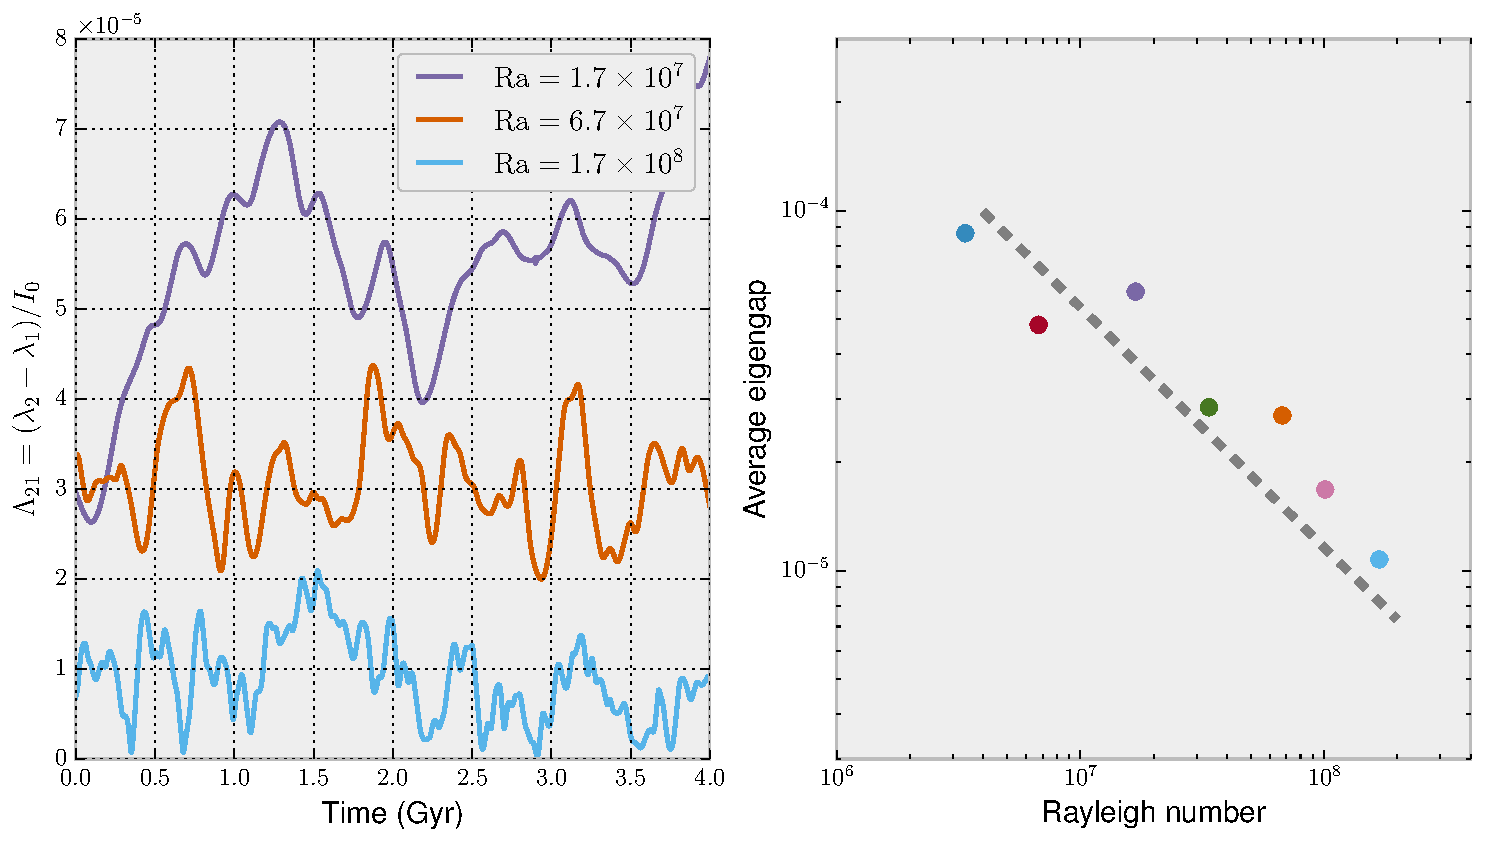
\includegraphics[width=0.9\textwidth]{figures/eigengap.pdf}
\caption{ Left: Time series of the normalized difference between moments $\Lambda_{12}$ for convection in a 2D annulus at several different Rayleigh numbers.  As the Rayliehg number increases, the average value of the relative moment decreases due to less low-degree coherence in the temperature structure.  Right:  average value of $\Lambda_{12}$ for the different Rayleigh numbers.  Also shown is a line with slope $\mathrm{Ra}^{-2/3}$, which is predicted from the scaling analysis (the exponent is $-2/3$ instead of $-1$ due to the reduced dimensionality of the simulations).}
\end{figure}

The nonhydrostatic moment of inertia is defined
\begin{equation}
J_{ij} = \int_{V_S} \rho \left( r_q r_q \delta_{ij} - r_i r_j \right) 
\end{equation}

where $V_S$ is the reference spherical volume of the mantle.
If we substitute in Equation \ref{eos} we find

\begin{equation}
J_{ij} = I_0 \delta_{ij} + \int_{V_S} \rho_0 \alpha T \left( r_q r_q \delta_{ij} - r_i r_j \right) = I_0 \delta_{ij} + E_{ij} 
\end{equation}

Nondimensionalizing the integral for $E_{ij}$ we find

\begin{equation}
J_{ij} = I_0 \delta_{ij} + \int_{V_S^\prime} \alpha T^\prime \left( r_q^\prime r_q^\prime \delta_{ij} - r_i^\prime r_j^\prime \right) 
\end{equation}


For thermal convection, the convective part of the moment of inertia $\bf E$ is directly related to the degree-two structure of the temperature field (see Appendix \ref{appendix:moments}).
Therefore, an estimate of one allows an estimate of the other.


The structure of thermal convection is primarily controlled by the Rayleigh number.  Once the Rayleigh number is sufficiently high ($\sim10^6$) 
the style of convection changes from steady/quasisteady to chaotic.  Accompanying this transition to chaos is a broadening of the spatial 
and temporal spectra \citep{mclaughlin1982transition}.  

We can expand the temperature structure of the convecting planet with a set of orthonormal basis functions $R_n Y_{lm}$, 
where $Y_{lm}$ are spherical harmonics, $R_n$ are some set of radial polynomials.  
\begin{equation} 
T( r , \theta, \phi, t )  = {\displaystyle \sum_{n=0}^\infty \sum_{l=0}^\infty \sum_{m=-l}^{l} } T_{lmn}(t) R_n(r) Y_{lm} (\theta , \phi)
\label{T_series}
\end{equation}

The quantity $\Lambda_{ij}$ is the normalized degree-two temperature field.  The temperature field has been normalized by $\Delta T$ and thus goes between zero and one, therefore the expansion in $X_{lmn}$ is constrained by

\begin{equation}
\lVert T(x,y,z, t) \rVert_\infty = \lVert {\displaystyle \sum_{n=0}^\infty \sum_{l=0}^\infty \sum_{m=-l}^{l} } T_{lmn}(t) R_n(r) Y_{lm} (\theta , \phi) \rVert_\infty = 1
\end{equation}

This is a strong constraint, but it gives very little information about the distribution of power across the $T_{lmn}$.  
We can, however, think about the power spectrum in two different regimes: that of steady/quasisteady flow (relatively low $\mathrm{Ra}$) and that of chaotic flow (relatively high $\mathrm{Ra}$).

At low Rayleigh number we expect the spectrum of the temperature field to be dominated by only a few low-degree modes (possibly, but not necessarily degree-two).

At high Rayleigh number we expect there to be a lengthscale which characterizes the smallest length of features in the convecting system.  
At lengthscales smaller than this diffusion will tend to wipe out heterogeneities, and there will be no power in those modes.  
Therefore we expect, to a good approximation, that we will be able to cut off the infinite sum in Equation \ref{T_series} at some maximum wavenumber, set by the smallest lengthscale $d$:
 
\begin{equation}
n_{\mathrm{max}}, l_{\mathrm{max}}, m_{\mathrm{max}} \sim \frac{R}{d}
\end{equation}

The total number of modes that are accessible to the system are therefore 

\begin{equation}
N_{\mathrm{modes}} = n_{\mathrm{max}} \times l_{\mathrm{max}} \times n_{\mathrm{max}} \sim \left( \frac{R}{d} \right)^{3}
\end{equation}

The value of each $T_{lmn}(t)$ will in general be some complex function of time, but for a given style of convection we expect there to be some average value.
For chaotic flow the power should be spread out amongst the modes accessible to it.
We may make the hypothesis that each of the modes are roughly as likely as any of the others, which implies

\begin{equation}
T_{\mathrm{degree 2}}(t) \sim \frac{1}{N_{\mathrm{modes}}} \sim \left( \frac{d}{R}\right)^3
\end{equation}

Any of a number of scaling laws can provide an estimate for the characteristic length scale of a convecting system which may depending on rheology, geometry, or density structure.
The simplest, based on boundary layer theory \citep{turcotte1967finite}, finds $d/R \sim \mathrm{Ra}^{-1/3}$, thus furnishing us with an estimate of the power in the degree-two part of the field as a function of Rayleigh number:

\begin{equation}
T_{\mathrm{degree 2}}(t) \sim \mathrm{Ra}^{-1}
\end{equation}

This result has a simple interpretation.  As the Rayleigh number of the system increases, the smallest lengthscale of convective features gets smaller.  The total power in the temperature field is spread across a larger spectrum, leaving less total power for the degree-two part, which is what drives TPW.

With an estimate for the power in the degree-two part of the temperature field, we may finally estimate $\Lambda_{ij}$:

\begin{equation}
\Lambda_{ij} \sim \frac{\Gamma}{\mathrm{Ra} }
\end{equation}


\subsection{An estimate of the mismatch $\theta$}

The mismatch between the current axis and the principle axis of the convective moment is perhaps the most important parameter in Equation \ref{scaled_rotation}.  
Much of the debate around the existence and magnitude of TPW on Earth comes down to the question of how big $\theta$ can be \citep{kirschvink1997evidence, steinberger1997changes}.

An estimate for $\theta$ must concern the stability of the convective moment of inertia. 
Convection is continuously redistributing mass throughout the mantle, which will perturb the convective moment of inertia.  
If the convective moment is stable to small perturbations, then $\theta$ should be small, but if it is not stable to perturbations, then $\theta$ could be up to $90^\circ$. 
Given a random perturbation to that moment, we would like to give a bound on how big the perturbation to $\theta$ is. 
This may be done by application of a theorem due to \citet{davis1970rotation}.

Let $\delta$ be the size of the perturbation to the convective moment of inertia tensor, and let $\lambda_3 \ge \lambda_2 \ge \lambda_1$ be the eigenvalues of that tensor.  
Then the rotation of the principal axes of the tensor is bounded by

\begin{equation}
\lVert \sin(2 \theta) \rVert \le \frac{ 2 \lVert \delta \rVert}{ \displaystyle \min_{i \neq j} \lVert \lambda_i - \lambda_j \rVert }
\label{eq:kahan}
\end{equation} 

That is to say, if there is a large difference between the eigenvalues, this stabilizes axes to perturbations.  
If, however, there is a small difference between the eigenvalues (i.e., they are nearly degenerate), then perturbations can cause large rotations of the principle axes.
This is illustrated in Figure \ref{fig:perturb}


We may arrive at a simple estimate of the growth rate of the angle $\theta$ by differentiating Equation \ref{eq:kahan}, tentatively holding $\lVert \lambda_i - \lambda_j \rVert$ fixed:

\begin{equation}
\lVert \dot{\theta} \rVert \le \frac{ \lVert \dot{\delta} \rVert}{ \displaystyle \min_{i \neq j} \lVert \lambda_i - \lambda_j \rVert }
\label{eq:grow_perturbation}
\end{equation} 

\begin{figure}
\centering
\label{fig:perturb}
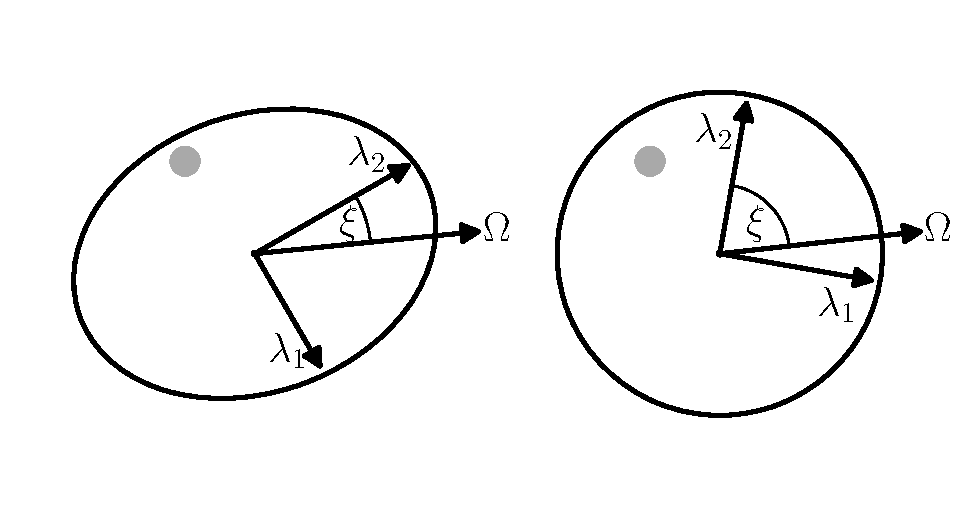
\includegraphics[width=0.9\textwidth]{figures/perturb.pdf}
\caption{Graphical demonstration of the $\sin{2 \theta}$ theorem of \citet{davis1970rotation}.  Two spheroidal bodies with eigenvalues $\lambda_2 > \lambda_1$ start out with the rotation axis $\Omega$ aligned with the $\lambda_2$ axis. However, on the left the eigengap $\lVert \lambda_2 - \lambda_1 \rVert$ is large, while on the right it is small.  A perturbation is instantaneously added to both bodies, which effects a small rotation of the principle axes on the left, but a large one on the right.}
\end{figure}


Furthermore, the quantity $(\lambda_i-\lambda_j)$ which appears in the denominator of these equations is precisely the same as the quantity which we estimated in the previous section to scale with $\sim \mathrm{Ra}^{-1}$.
Therefore, as the Rayleigh number increases, the characteristic gap between the eigenvalues of the convective moment becomes smaller.  
Additionally, the timescale of fluctuations in these values goes down. 
Overall, this makes the principle axes of high Rayleigh number systems much less stable.
This is consistent with the result of \citet{richards1999polar}.

In the limit that the eigengap becomes zero, the rotation of the pinciple axes can be arbitrary. 
This essentially corresponds to the hypothesized ``inertial interchange true polar wander'' \citep{kirschvink1997evidence}.

\begin{figure}
\centering
\label{misfit}
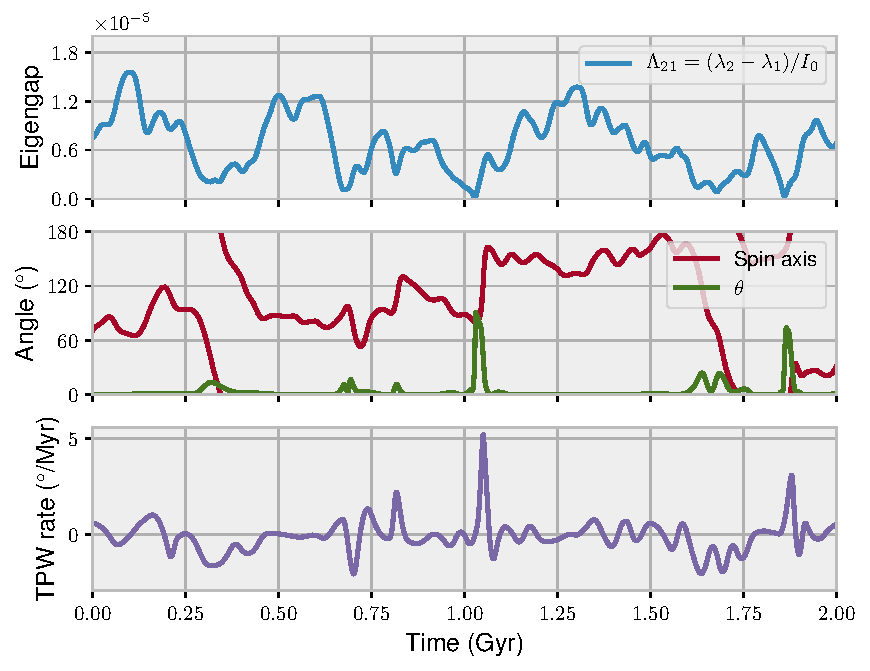
\includegraphics[width=0.9\textwidth]{figures/misfit.pdf}
\caption{Top: Time series of principle moments for 2D annular convection at $\mathrm{Ra}\sim10^8$.  Bottom: Time series of spin axis and mismatch angle $\theta$.  When the two moments are close to each other (small eigengap), the mismatch angle becomes large, and the rate of polar wander is significantly larger.}
\end{figure}



\section{Discussion}

The preceding results clarify the complex relationship between the Rayleigh number, the Froude number and the rates of TPW for a convecting planet.
As mantle convection redistributes mass in the planet's interior, the rotational bulge moves around to stay aligned with the principle axes of the convective moment of inertia. 
There is a constant competition between growth of the mismatch angle $\theta$ through Equation \ref{eq:grow_perturbation} and its relaxation through Equation \ref{simple_milankovitch}.
We may plug in the estimate for $\Lambda_{ij}$ into equation \ref{simple_milankovitch} to find the strikingly simple expression
\begin{equation}
\frac{\kappa}{R^2} \; \dot{\theta} \sim -\frac{1}{\mathrm{Fr}} \sin{2 \theta}
\label{eq:simplest_milankovitch}
\end{equation}
Surprisingly, $\Gamma$ and $\mathrm{Ra}$ have completely dropped from the scaling. 
This is somewhat of a coincidence due to the simple estimate of the smallest lengthscales of the problem.
However, we expect that more complicated estimates for $d(\mathrm{Ra})$ will still show a weak dependence on the Rayleigh number.

More important is the observation that the most important parameters are the Froude number, which acts as the brakes on the system, and $\theta(\mathrm{Ra})$.
Whereas the rest of the expression has at most a weak dependence on $\mathrm{Ra}$, this is expected to be strongly dependent on it.

Indeed, we can identify two endmember behaviors of Equation \ref{eq:simplest_milankovitch}.
When convection is not sufficiently chaotic to create a large $\theta$ we are in the regime where the planet's rotation axis closely tracks that of the convective moment.
This is the regime considered in \citet{steinberger1997changes}, \citet{roberts2007cause}, and \citet{zhong2007supercontinent}, and can be considered the ``slow TPW'' regime.

When convection is more chaotic, however, there may be large excursions in $\theta$, which can drastically increase the wander rate.  
If $\theta=90^\circ$, this corresponds to IITPW \citep{kirschvink1997evidence}.  
This, however, is a special case in the large $\theta$, ``fast TPW'' regime.



\section{Conclusion}
We have developed a framework for discussing the rates of true polar wander in terms of a small number of nondimensional numbers.


\begin{acknowledgments}
\end{acknowledgments}

\bibliographystyle{gji}
\bibliography{tpw_rate.bib}


\appendix

\section{Degree-two moments}
\label{appendix:moments}

We may explicitly draw a connection between the moment of inertia of a rotating object and it's degree-two density structure.  The moment of inertia tensor may be written in index notation
\begin{equation}
I_{ij} = \int_V \rho \left( r_q r_q \delta_{ij} - r_i r_j \right) d^3 {\bf r}
\label{inertia}
\end{equation}

where $\bf r$ is the Eulerian coordinate, $\rho$ is the density, and $V$ is the volume of the material.  The degree-two density structure may be expressed as a quadrupole-moment tensor (cf. \citet{jackson1998classical}):

\begin{equation}
Q_{ij} = \int_V \rho \left( 3 r_i r_j - r_q r_q \delta_{ij} \right) d^3 {\bf r}
\end{equation}

The commutator of these tensors, $\bf QI - IQ$, is zero, indicating that they may be simultaneously diagonalized.  

\ifdetail
We may demonstrate that the commutator is zero by using the definition of the commutator and expanding:
\begin{equation} 
\begin{aligned}
{\bf IQ-QI} = &I_{ik} Q_{kj} - Q_{ik} I_{kj} \\
 = &\int_V \rho \left( r_q r_q \delta_{ik} - r_i r_k \right) d^3 {\bf r} \int_V \rho \left( 3 r_k r_j - r_q r_q \delta_{kj} \right) d^3 {\bf r} \\
 &- \int_V \rho \left( r_q r_q \delta_{kj} - r_k r_j \right) d^3 {\bf r} \int_V \rho \left( 3 r_i r_k - r_q r_q \delta_{ik} \right) d^3 {\bf r} \\
 = &3 \delta_{ik} \int_V \rho r_q r_q d^3 {\bf r} \int_V \rho r_k r_j d^3 {\bf r} \\
 &-\delta_{kj} \delta_{ik} \int_V \rho r_q r_q d^3 {\bf r} \int_V \rho r_q r_q d^3 {\bf r} \\
 &-3 \int_V \rho r_i r_k d^3 {\bf r} \int_V \rho r_k r_j d^3 {\bf r} \\
 &+\delta_{kj} \int_V \rho r_i r_k d^3 {\bf r} \int_V \rho r_q r_q d^3 {\bf r} \\
 - &3 \delta_{kj} \int_V \rho r_q r_q d^3 {\bf r} \int_V \rho r_i r_k d^3 {\bf r} \\
 &+\delta_{ik} \delta_{kj} \int_V \rho r_q r_q d^3 {\bf r} \int_V \rho r_q r_q d^3 {\bf r} \\
 &+3 \int_V \rho r_k r_j d^3 {\bf r} \int_V \rho r_i r_k d^3 {\bf r} \\
 &-\delta_{ik} \int_V \rho r_k r_j d^3 {\bf r} \int_V \rho r_q r_q d^3 {\bf r} \\
 = \;&3 \int_V \rho r_q r_q d^3 {\bf r} \int_V \rho r_i r_j d^3 {\bf r} \\
 &+ \int_V \rho r_i r_j d^3 {\bf r} \int_V \rho r_q r_q d^3 {\bf r} \\
 - &3 \int_V \rho r_q r_q d^3 {\bf r} \int_V \rho r_i r_j d^3 {\bf r} \\
 &- \int_V \rho r_i r_j d^3 {\bf r} \int_V \rho r_q r_q d^3 {\bf r} \\
 & = 0
\end{aligned}
\end{equation}
\else
\fi

We may therefore go into the principle coordinate system of both tensors to find
\begin{equation}
{\bf I} = {\bf 1} \begin{bmatrix}
\int_V \rho (y^2+z^z)\\
\int_V \rho (x^2+z^2) \\
\int_V \rho (x^2+y^2) 
\end{bmatrix}
\end{equation}

\begin{equation}
{\bf Q} = {\bf 1} \begin{bmatrix}
\int_V \rho (2 x^2 - y^2 - z^z)\\
\int_V \rho (2 y^2 - x^2 -z^2)\\
\int_V \rho (2 z^2 - x^2 - y^2) 
\end{bmatrix}
\end{equation}

where $\bf 1$ is the identity matrix.  If we let the diagonal elements of $\bf I$ be $\lambda_1, \lambda_2, \lambda_3$, we may rewrite $\bf Q$ as

\begin{equation}
{\bf Q} = {\bf 1} \begin{bmatrix}
(\lambda_2-\lambda_1) + (\lambda_3-\lambda_1)\\
(\lambda_1-\lambda_2) + (\lambda_3-\lambda_2)\\
(\lambda_1-\lambda_3) + (\lambda_2-\lambda_3)\\
\end{bmatrix}
\label{maccullagh}
\end{equation}

which shows the connection between the degree-two component of the density field and the principle moments of inertia.  This may be seen as a form of MacCullagh's formula \citep{munk1960rotation}.


\section {TODO}

\begin{enumerate}
\item Figure out the best way of nondimensionalizing ($\alpha \Delta T$)
\item Connect nondimensionalization with Equation \ref{eq:liouville} via correspondence principle
\item Make notation everywhere consistent
\item More discussion of Davis+Kahan?
\item Make better figures
\item Integrate numerical results
\item Make the argument about degree-two scaling much sharper
\item Can I write equation \ref{eq:liouville} in terms of \ref{maccullagh}?
\item Discuss elastic lithosphere, Creveling
\item Discuss high-viscosity lower mantle
\item Earth-like parameters
\end{enumerate}

\label{lastpage}

\end{document}
